% !TEX program = xelatex
\documentclass[10pt,a4paper]{ctexart}

% ==================== Packages ====================
\usepackage[top=2.5cm, bottom=2.5cm, left=2.8cm, right=2.8cm]{geometry}
\usepackage{graphicx}
\usepackage{booktabs}
\usepackage{amsmath}
\usepackage{amssymb}
\usepackage{hyperref}
\usepackage{caption}
\usepackage{subcaption}
\usepackage{enumitem}
\usepackage{fancyhdr}
\usepackage{titlesec}
\usepackage{xcolor}
\usepackage{float}
\usepackage{longtable}
\usepackage{array}
\usepackage{multirow}

\hypersetup{
    colorlinks=true,
    linkcolor=blue,
    urlcolor=blue,
    citecolor=blue
}

% ==================== Styling ====================
\setlength{\headheight}{14pt}
\pagestyle{fancy}
\fancyhf{}
\fancyhead[L]{\small 深度学习基础大作业}
\fancyhead[R]{\small 股票趋势预测与模拟交易}
\fancyfoot[C]{\thepage}
\renewcommand{\headrulewidth}{0.4pt}

\titleformat{\section}{\Large\bfseries}{\thesection}{1em}{}
\titleformat{\subsection}{\large\bfseries}{\thesubsection}{1em}{}

\definecolor{upgreen}{RGB}{0,128,0}
\definecolor{downred}{RGB}{200,30,30}

% ==================== Title ====================
\title{
    \vspace{0.4cm}
    {\Huge\bfseries 基于深度学习的\\[0.25cm] 股票趋势预测与模拟交易}\\[0.6cm]
}
\author{
    \begin{tabular}{c}
        李佳乐\quad 刘世阳
    \end{tabular}
}
\date{\today}
\renewcommand{\abstractname}{\Large\textbf{摘\quad 要}}

\begin{document}

\maketitle
\thispagestyle{empty}

% ==================== Abstract ====================
\begin{abstract}
本实验面向A股日频量化选股场景，围绕“能否稳定给出截面排序”而不是单点拟合，构建了 \textbf{EnsembleAttentionGRU + HybridLoss} 的端到端流程。模型输入57维多源特征，预测T+5日累计收益率；在2025年验证集上取得\textbf{+55.02\%总收益}和\textbf{3.12}的夏普比率。2026年6月1--12日的模拟交易结果为\textbf{-1.35\%}，但调仓记录显示模型对新易盛、中际旭创、天孚通信等AI算力主线具备明确识别能力，回撤主要来自行业集中、短期风格切换以及比赛满仓约束下无法启用回测中的MA60风控过滤。实验结论并不是“模型无效”，而是该模型更适合作为一个可用的选股排序器，而非在所有市场状态下都能独立生成稳定收益的完整交易系统。

\par\textbf{关键词：}深度学习；股票预测；GRU；Attention；集成学习；HybridLoss；模拟交易
\end{abstract}

\newpage
\setcounter{page}{1}
\tableofcontents
\newpage

% ======================================================================
\section{数据处理与问题定义}
% ======================================================================

\subsection{股票池选择}

依据作业要求，我们先排除了北交所和ST、\*ST股票，再将研究范围收缩到\textbf{沪深300 + 中证500成分股}。这个选择并不是单纯为了减少样本量，而是为了在可计算性、流动性和噪声水平之间取得更合理的平衡：成分股的成交更连续、财务指标缺失更少，模型更容易学习到可重复的截面排序；相比之下，全市场小微盘股票虽然数量更大，但停牌、极端波动和结构性缺失会显著放大训练噪声。对这个任务而言，\textbf{样本质量比样本数量更重要}，因为我们追求的是稳定的排序能力，而不是对少数极端样本的记忆。

\subsection{数据来源与维度}

模型并不是只看单一行情表，而是把日频量价、估值和资金流向拼成一个统一视图。这样做的目的，是让后续特征工程围绕“价格怎么走、资金是否认可、估值处在什么位置”三个问题展开，而不是把模型限制在纯价格序列上。

\begin{table}[htbp]
    \centering
    \caption{数据来源一览}
    \footnotesize
    \begin{tabular}{p{2.3cm}p{2.6cm}p{6.8cm}p{2.0cm}}
        \toprule
        数据类别 & 来源目录 & 核心字段 & 时间范围 \\
        \midrule
        日频量价 & \texttt{daily/} & open, high, low, close, pct\_chg, vol, amount, vwap & 2016--2026 \\
        基本面指标 & \texttt{metric/} & pe\_ttm, pb, ps\_ttm, circ\_mv, total\_mv & 同上 \\
        资金流向 & \texttt{moneyflow/} & 小/中/大/特大单买卖量价, net\_mf\_amount & 同上 \\
        指数成分 & \texttt{index\_weight/} & 沪深300/中证500成分股列表 & --- \\
        ST标记 & \texttt{stock\_st/} & 每日ST列表 & --- \\
        \bottomrule
    \end{tabular}
\end{table}

\subsection{数据预处理}

\textbf{（1）缺失值处理}

缺失值主要来自停牌、新股上市时间不一致、早期资金流向数据覆盖不足以及亏损公司估值字段为空。我们按股票分组做前向填充，再将仍缺失的值置0。前向填充的含义是：在没有新披露或没有新交易的日期，模型只能沿用最近一次可观察状态；这与真实交易中“无法看到未来数据”的信息条件一致。对于资金流向和估值字段，置0并不表示其经济含义为0，而是将“无可用增量信息”显式编码给模型，避免因为删除样本进一步降低股票覆盖度。

\textbf{（2）板块时间过滤}

不同板块的涨跌停制度不同，会改变收益率分布和交易可行性。创业板在2020-08-24后涨跌幅限制由10\%调整为20\%，此前样本与此后样本不完全服从同一交易制度；如果直接混合训练，模型可能把制度变化误学成个股风险特征。因此我们对创业板做制度切换后的时间过滤：
\begin{itemize}
    \item 创业板（300开头）：仅使用\textbf{2020-08-24}之后数据（此前涨跌幅为10\%，此后改为20\%）
    \item 其他板块（主板/科创板）：使用2016-01-01之后数据
\end{itemize}

\textbf{（3）标准化方案}

采用\textbf{训练集拟合、全时期应用}的标准化方案：只在训练集上计算每个特征的均值和标准差，再应用于验证集、测试集和比赛期预测数据。该方案牺牲了一部分对未来市场分布变化的自适应能力，但换来了更清晰的防泄露边界。由于训练期覆盖2016--2024年，统计量跨越多轮市场周期，足以作为稳定尺度；验证集和比赛期仅被动接受该尺度，不参与任何参数估计。

$$ \mu = \frac{1}{N_{train}}\sum_{i \in train} x_i, \quad \sigma = \sqrt{\frac{1}{N_{train}}\sum_{i \in train}(x_i - \mu)^2}, \quad x_i' = \frac{x_i - \mu}{\sigma} $$

\subsection{特征工程}

特征工程的目标不是简单堆叠指标，而是将原始行情转换为模型更容易识别的“相对状态”。57维特征可以分为三类：第一类是价格、成交量和技术指标，用于刻画短期趋势、动量和波动；第二类是估值、市值等慢变量，用于刻画风格暴露和估值位置；第三类是资金流向及其衍生指标，用于刻画交易行为是否支持价格变化。三类信息的时间尺度不同，正好与GRU处理短序列时的多维输入结构匹配。

\begin{table}[htbp]
    \centering
    \caption{特征体系概览}
    \footnotesize
    \begin{tabular}{lll}
        \toprule
        类别 & 代表性特征 & 特征数 \\
        \midrule
        原始量价 & open, high, low, close, pre\_close, pct\_chg & 6 \\
        成交量/额 & vol, amount, vwap, change & 4 \\
        基本面 & pe\_ttm, pb, ps\_ttm, circ\_mv, total\_mv等 & 14 \\
        资金流向 & buy/sell\_sm/md/lg/elg\_vol/amount, net\_mf\_amount等 & 16 \\
        移动均线 & ma5, ma10, ma20 & 3 \\
        价格动量 & mom5, mom10 & 2 \\
        波动率 & volatility20 & 1 \\
        成交量均线 & vol\_ma5 & 1 \\
        技术指标 & macd, rsi14 & 2 \\
        资金流衍生 & net\_mf\_amount\_ma5, mf\_to\_amount\_ratio & 2 \\
        PE衍生 & pe\_ttm\_ma60, pe\_ttm\_deviation & 2 \\
        市值衍生 & log\_circ\_mv & 1 \\
        其他 & turnover\_rate\_f, volume\_ratio, dv\_ttm & 3 \\
        \midrule
        \textbf{合计} & & \textbf{57} \\
        \bottomrule
    \end{tabular}
\end{table}

其中三个特征对任务尤其关键。其一，\texttt{mf\_to\_amount\_ratio = net\_mf\_amount / amount} 将净流入额除以成交额，避免大市值股票天然拥有更大资金流金额，从而提升不同股票之间的可比性；\texttt{net\_mf\_amount\_ma5} 则把单日资金冲击转换为短期资金趋势。其二，\texttt{pe\_ttm\_deviation} 衡量当前估值相对60日均值的偏离，它并不直接预测“低估必涨”，而是为模型提供估值扩张或回归的上下文。其三，\texttt{log\_circ\_mv} 用对数压缩市值长尾分布，使模型能够学习大盘/中盘风格，而不被少数超大市值股票主导梯度。

\subsection{标签构造与预测目标}

预测目标为\textbf{T+5日累计收益率}（基于\texttt{pct\_chg}字段）：

\begin{equation}
    y_t = \sum_{i=1}^{5} r_{t+i}
\end{equation}

实现方式为对每只股票将\texttt{pct\_chg}前移一期，再计算5日滚动和并对齐到当前样本。这样构造后，时点$t$的输入窗口只包含$t$及以前的信息，标签覆盖$t+1$到$t+5$的未来收益。

选择T+5而不是T+1，是因为本任务最终服务于Top-N持仓策略，而不是日内方向判断。单日收益中噪声占比很高，容易导致模型围绕随机涨跌过拟合；5日累计收益能平滑一部分微观扰动，也与“每天只换少量持仓”的策略节奏更一致。换句话说，标签的选择与交易周期共同定义了模型要学习的信号：它更关注短期趋势能否延续，而不是预测明天是否上涨。

\subsection{数据集划分与防泄露设计}

\textbf{时间划分}（严格时序，禁止随机打乱）：

\begin{table}[htbp]
    \centering
    \caption{数据集划分}
    \begin{tabular}{lll}
        \toprule
        数据集 & 时间范围 & 规模 \\
        \midrule
        训练集 & 2016-01 $\sim$ 2024-12 & $\sim$51万行，291只股票 \\
        验证集 & 2025-01 $\sim$ 2025-12 & $\sim$7万行，293只股票 \\
        测试集 & 2026-01 $\sim$ 2026-05 & $\sim$2.8万行，293只股票 \\
        比赛期 & 2026-06-01 $\sim$ 2026-06-12 & --- \\
        \bottomrule
    \end{tabular}
\end{table}

滑动窗口长度设为15个交易日，输入为$X_{[t-14:t]} \in \mathbb{R}^{15 \times 57}$，标签为$y_t$。15天窗口覆盖约三周交易，足以包含短期趋势、放量突破和均线变化，又不会像60天长窗口那样显著增加参数记忆压力。窗口通过\texttt{stock\_changes}识别股票边界，严格保证不跨股票拼接。

防泄露设计贯穿整个数据流：数据集按时间划分，训练集永远早于验证集和测试集；标准化参数只由训练集拟合；技术指标全部使用rolling或ewm形式，只依赖当日及历史值；标签虽然使用未来收益，但只作为监督信号，不进入输入特征；滑动窗口只在同一只股票内部构造。这些约束使得历史回测更接近真实比赛中的信息条件。

% ======================================================================
\section{模型实现}
% ======================================================================

\subsection{整体架构：EnsembleAttentionGRU}

最终模型采用3个AttentionGRU子模型并行集成，如图\ref{fig:model_arch}所示。三个分支接收相同的$15\times57$输入，但参数独立初始化、独立产生预测分数，最后对三个标量预测取平均。这个设计针对的是金融序列预测中最突出的问题：信号弱、噪声强，单个模型很容易因为初始化和局部样本波动给出不稳定排序。均值集成不会改变模型的主要归纳偏置，但可以降低预测方差，使Top-N股票列表在相邻训练轮次和相邻交易日之间更稳定。

\begin{figure}[htbp]
    \centering
    \begin{subfigure}[t]{0.47\textwidth}
        \centering
        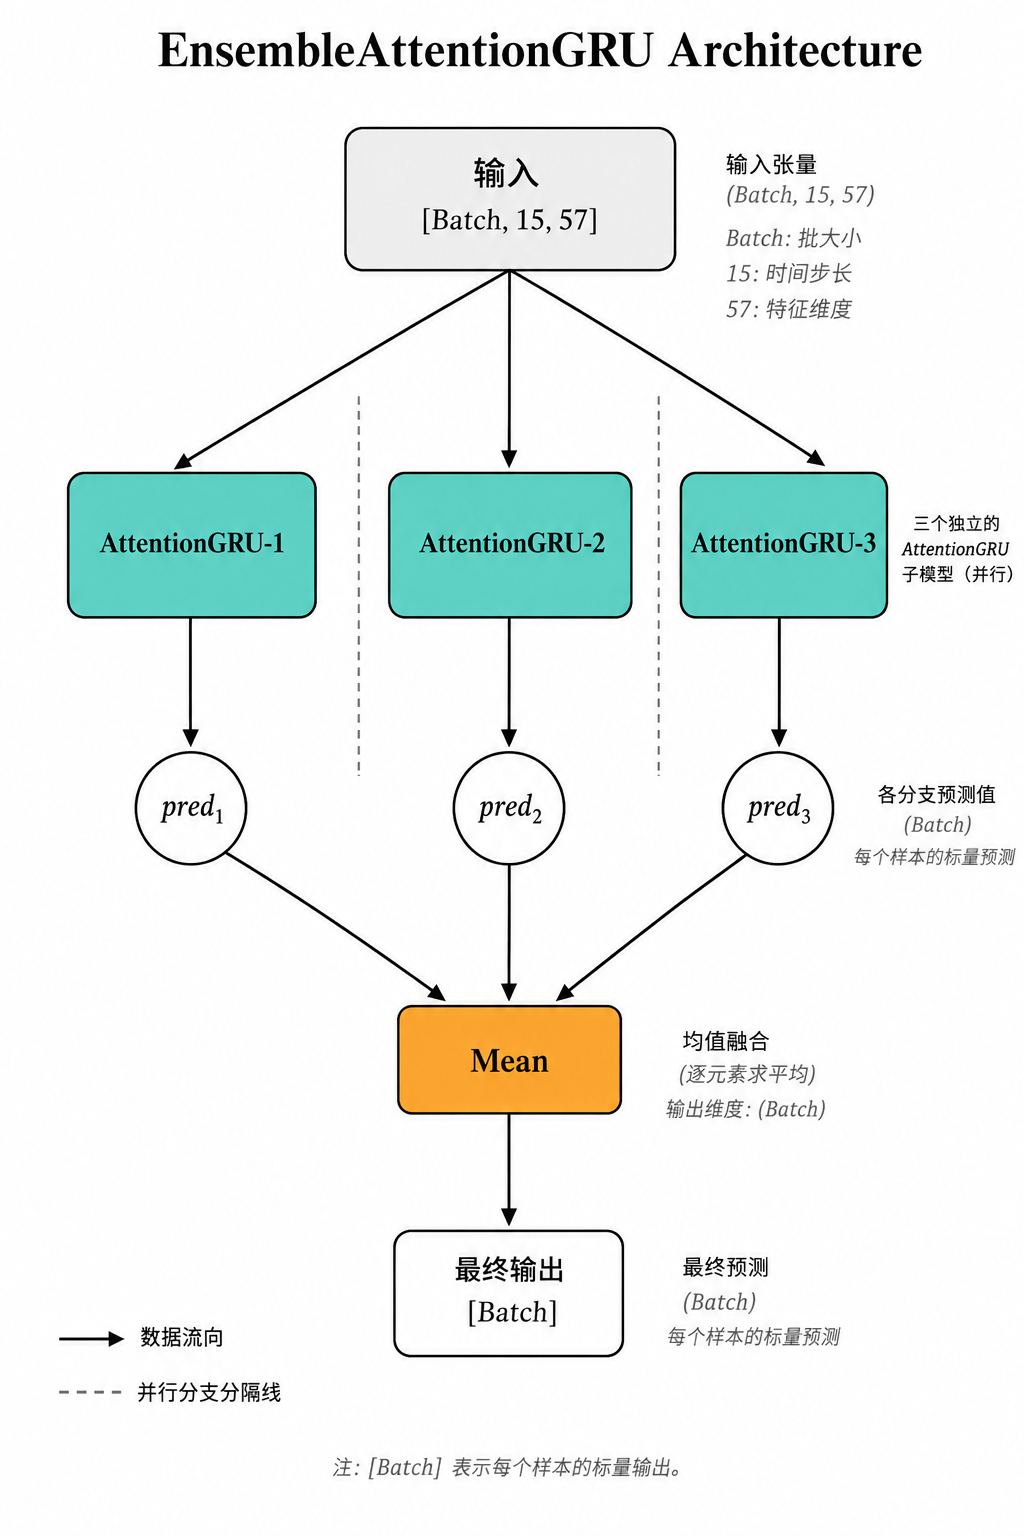
\includegraphics[width=\linewidth,height=0.43\textheight,keepaspectratio]{figures/ensemble_architecture.png}
        \caption{EnsembleAttentionGRU整体架构}
        \label{fig:ensemble_arch}
    \end{subfigure}
    \hfill
    \begin{subfigure}[t]{0.47\textwidth}
        \centering
        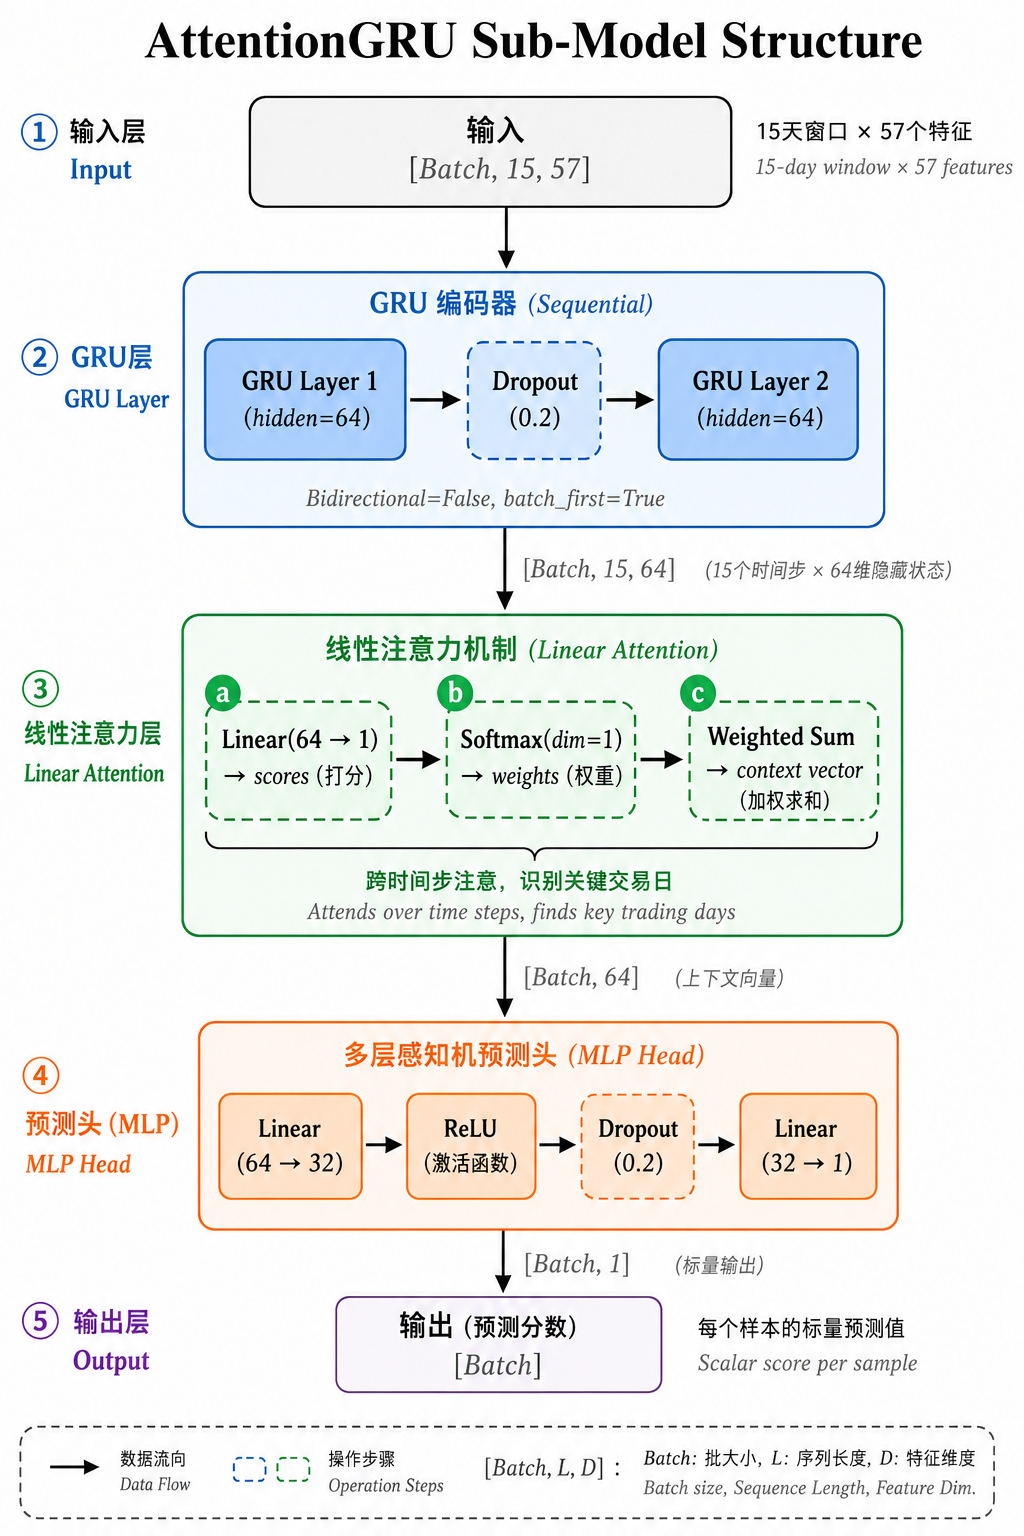
\includegraphics[width=0.86\linewidth,height=0.38\textheight,keepaspectratio]{figures/attention_gru.png}
        \caption{AttentionGRU子模型内部结构}
        \label{fig:attention_gru}
    \end{subfigure}
    \caption{模型架构示意图}
    \label{fig:model_arch}
\end{figure}

模型总参数量为\textbf{152,259}，三个子模型各约50,753个参数。与更深的Transformer或大规模双向RNN相比，这个参数规模较小，但更适合本实验的数据条件：股票日频数据虽然样本行数不少，真正可复用的信号却很弱，过大的模型更容易提升训练集拟合而不是提升样本外IC。

\subsection{AttentionGRU子模型}

每个子模型由单向GRU、线性注意力和两层MLP预测头组成，结构如图\ref{fig:attention_gru}所示。GRU负责把15天窗口编码为一串隐状态；注意力层在时间维度上分配权重，将不同交易日的信息压缩为一个上下文向量；MLP头再把上下文向量映射为标量预测分数。这样的结构与任务目标相匹配：我们不需要逐日输出，而只需要对当前样本给出一个可用于截面排序的分数。

各组件的取舍如下。GRU相比LSTM少一个门控结构，参数更少，在15步短序列上表达能力已经足够；hidden size设为64，是因为更大的隐藏维度在迭代中没有带来稳定IC提升，反而增加了样本外波动；注意力层采用Linear Attention而不是Multi-Head Attention，是因为输入窗口较短，多头结构增加的自由度主要会放大噪声；预测头只使用$64 \rightarrow 32 \rightarrow 1$的浅层MLP，以保留必要非线性但避免过参数化。

\begin{table}[htbp]
    \centering
    \caption{模型组件设计选择}
    \small
    \begin{tabular}{p{2.5cm}p{3.5cm}p{7.0cm}}
        \toprule
        组件 & 设计选择 & 理由 \\
        \midrule
        时序编码器 & GRU（非LSTM） & 参数更少，在15步序列上效果相当 \\
        隐藏维度 & 64（非128/256） & 更大hidden size IC提升有限但方差增大 \\
        注意力机制 & Linear Attention & 15天序列长度较短，简单注意力已足够 \\
        MLP Head & $64\to32\to1$ + ReLU & 适度的非线性增强，避免过参数化 \\
        正则化 & Dropout + WD & Dropout=0.2，Weight Decay=$10^{-5}$，用于降低低信噪比数据上的过拟合 \\
        \bottomrule
    \end{tabular}
\end{table}

\subsection{损失函数：HybridLoss}

如果只用MSE，模型优化的是预测值与真实收益的数值距离；但交易策略真正使用的是预测分数的相对排名。为此，本实验采用\textbf{MSE + Pairwise Ranking Loss}的组合损失：

\begin{equation}
    \mathcal{L} = \alpha \cdot \mathcal{L}_{MSE} + (1-\alpha) \cdot \mathcal{L}_{Rank}
\end{equation}

其中$\alpha = 0.5$。

MSE部分保留收益幅度信息，防止模型只学到相对顺序而完全失去分数尺度：
\begin{equation}
    \mathcal{L}_{MSE} = \frac{1}{N}\sum_{i=1}^{N}(pred_i - y_i)^2
\end{equation}

Pairwise Ranking部分在每日截面内采样股票对$(i, j)$。当$|y_i-y_j|>0.001$时，说明两只股票未来5日收益差异超过0.1\%，排序关系具有一定意义；此时损失要求预测分数差与真实收益差同号：
\begin{equation}
    \mathcal{L}_{pair} = \mathrm{softplus}(-\mathrm{sign}(y_i - y_j) \cdot (pred_i - pred_j))
\end{equation}

这里的\texttt{target\_margin = 0.001}相当于一个噪声过滤器：收益率差异过小的股票对本身难以区分，强行排序只会把随机扰动写进梯度。\texttt{max\_pairs\_per\_day = 1000}则控制计算复杂度，避免某些交易日股票对数量过大导致训练不稳定。最终$\alpha=0.5$表示数值拟合和排序约束各占一半，使训练目标既贴近回归标签，又服务于Top-N选股策略。

\subsection{训练配置与版本演进}

\begin{table}[htbp]
    \centering
    \caption{训练超参数}
    \begin{tabular}{ll}
        \toprule
        超参数 & 值 \\
        \midrule
        优化器 & Adam \\
        学习率 & $1\times10^{-3}$ \\
        Weight Decay & $1\times10^{-5}$ \\
        Batch Size & 12,288 \\
        Epochs（实验） & 15 + early stopping (patience=5) \\
        Epochs（比赛） & 2 \\
        随机种子 & 42 \\
        \bottomrule
    \end{tabular}
\end{table}

实验经历了多轮迭代，逐步收敛到v4.2最终方案。早期版本更强调模型容量和全市场覆盖，后期版本转向控制噪声、提升排序稳定性：

\begin{table}[htbp]
    \centering
    \caption{版本演进历程}
    \small
    \begin{tabular}{p{2.0cm}p{9.0cm}p{3.0cm}}
        \toprule
        版本 & 关键改进 & 验证集IC \\
        \midrule
        v1 (MVP) & 基础GRU + Attention, MLP基线 & $\sim$0.04 \\
        v2 & T+5预测目标 + HybridLoss引入 & $\sim$0.06 \\
        v3 & 全量股票池, 特征扩展至47维 & $\sim$0.05 \\
        v4 & 双向GRU + 超参数调优 & $\sim$0.095 \\
        \textbf{v4.2} & \textbf{Ensemble集成(3模型), 57维特征, CS300+500池} & \textbf{$\sim$0.06（更稳定）} \\
        \bottomrule
    \end{tabular}
\end{table}

需要说明的是，v4的单次验证IC更高，但它依赖更复杂的结构和更宽的股票池，回测与后续比赛预测的稳定性并不理想。v4.2选择“较低但更稳”的IC：单模型改为三模型集成，双向GRU改为单向GRU，全量股票池收缩到沪深300+中证500，并补充资金流衍生和PE偏离度等特征。这一变化体现了本实验后期的核心判断：在金融数据中，泛化稳定性比追求某一次验证指标峰值更重要。

% ======================================================================
\section{模型评估与历史回测}
% ======================================================================

\subsection{训练过程与损失收敛}

实验阶段模型在训练集（2016--2024）上训练，在验证集（2025）上做早停。由于HybridLoss的绝对数值混合了MSE和排序项，直接比较训练/验证损失并不能完全反映选股质量；因此训练时更关注验证集相关性指标，正式评估时再按交易日计算截面Rank IC。这个选择与任务目标一致：我们最终关心的不是预测收益率小数点后是否精确，而是模型能否把未来表现更好的股票排在更前面。

\begin{table}[htbp]
    \centering
    \caption{训练过程关键节点}
    \begin{tabular}{lll}
        \toprule
        Epoch & 验证Rank IC & 备注 \\
        \midrule
        1 & \textbf{0.0639} & \textbf{Best IC，保存最优权重} \\
        2 & $\sim$0.058 & 开始波动 \\
        $\cdots$ & $\cdots$ & $\cdots$ \\
        13 & --- & Early Stopping触发 \\
        \bottomrule
    \end{tabular}
\end{table}

模型在13 epoch时触发早停，最优checkpoint对应epoch 1的Val IC = 0.0639。这一现象看似“训练过早达到最好”，但在金融时间序列中并不反常：个股未来收益中随机成分很高，模型很快可以学到最粗粒度的动量、资金流和风格信号，继续训练则更容易拟合特定年份、特定行业的噪声。早停的作用就是在“学到可泛化结构”和“记住训练期细节”之间截断。

比赛阶段在全量可用数据（2016--2026.5）上训练2 epoch，损失从$\sim$0.443降至$\sim$0.430。我们没有在比赛前进行长轮次训练，原因是比赛期没有独立验证标签，过度训练只会提高对历史最新阶段的拟合，不一定提高未来10个交易日的泛化。

\subsection{基础评估指标（IC / ICIR）}

在验证集（2025年）上逐日计算预测分数与T+5收益率的截面Spearman相关系数：

\begin{table}[htbp]
    \centering
    \caption{IC/ICIR评估结果}
    \begin{tabular}{lcc}
        \toprule
        指标 & 验证集(2025) & 测试集(2026.1--5) \\
        \midrule
        \textbf{Rank IC Mean} & \textbf{0.0596} & -0.0090 \\
        Rank IC Std & 0.1193 & 0.1307 \\
        \textbf{ICIR} & \textbf{0.4995} & -0.0690 \\
        \textbf{IC $>$ 0 比例} & \textbf{68.31\%} & 50.00\% \\
        \bottomrule
    \end{tabular}
\end{table}

验证集Rank IC均值为0.0596，ICIR接近0.5，且68.31\%的交易日IC为正，说明模型在2025年具有较稳定的截面排序能力。这里的“稳定”不是指每天都能盈利，而是指在多数交易日里，预测分数与未来5日收益存在正相关。对于Top-N策略而言，这已经足以形成组合层面的统计优势。

测试集2026年1--5月的Rank IC降至-0.0090，说明模型在最新市场环境中的排序优势明显衰减。这一结果非常重要：它提前暴露了比赛可能遇到的风格切换风险，也提醒我们不能只用2025年回测成功来证明策略一定有效。后续比赛出现高波动和回撤，本质上与这个样本外IC衰减是相互印证的。

\subsection{回测设置}

\begin{table}[htbp]
    \centering
    \caption{回测参数配置}
    \begin{tabular}{ll}
        \toprule
        参数 & 值 \\
        \midrule
        初始资金 & \yen1,000,000 \\
        持仓数量(n) & 20只，等权 \\
        每日调仓(k) & 2只 \\
        交易成本 & 买入0.025\%佣金；卖出0.025\%佣金+0.05\%印花税 \\
        滑点 & 0.1\% \\
        T+1机制 & 当日买入次日可卖 \\
        涨跌停限制 & 涨停不可买入，跌停不可卖出 \\
        最小交易单位 & 主板100股，科创板200股 \\
        仓位要求 & 满仓操作 \\
        \bottomrule
    \end{tabular}
\end{table}

\subsection{验证集回测（2025年）}

\begin{table}[htbp]
    \centering
    \caption{验证集回测结果}
    \begin{tabular}{ll}
        \toprule
        指标 & 结果 \\
        \midrule
        回测区间 & 2025-04-07 $\sim$ 2025-12-31（183交易日） \\
        \textbf{总收益率} & \textbf{+55.02\%} \\
        \textbf{年化收益率} & \textbf{+82.89\%} \\
        \textbf{夏普比率} & \textbf{3.12} \\
        最大回撤 & -9.07\% \\
        日胜率 & 60.11\% \\
        \bottomrule
    \end{tabular}
\end{table}

2025年验证集回测表现较好，原因有两层。第一，模型在该时期的Rank IC为正且正IC比例较高，说明选股信号本身有效；第二，2025年市场结构有利于模型偏好的科技成长方向，尤其是AI算力、半导体、PCB等板块表现较强。换言之，+55.02\%收益并不能完全归因于模型“预测得准”，它同时受益于市场主线与模型选股偏好的匹配。因此我们更重视夏普比率和最大回撤：夏普为3.12、最大回撤为-9.07\%，说明收益并非只来自少数极端交易日，而是具有较好的风险调整后表现。

\subsection{测试集回测（2026年1--5月）}

\begin{table}[htbp]
    \centering
    \caption{测试集回测结果}
    \begin{tabular}{ll}
        \toprule
        指标 & 结果 \\
        \midrule
        回测区间 & 2026-01-02 $\sim$ 2026-05-13（23交易日） \\
        \textbf{总收益率} & \textbf{+1.72\%} \\
        年化收益率 & +20.52\% \\
        夏普比率 & 1.08 \\
        最大回撤 & -2.02\% \\
        \bottomrule
    \end{tabular}
\end{table}

测试集只有23个交易日，年化收益和夏普比率不宜过度解读。从绝对收益看，策略仍取得+1.72\%，但IC指标已经接近随机，说明这段收益可能更多依赖组合持仓与短期市场波动的偶然匹配。我们据此将测试集结果视为“风险提示”而不是“强验证”：模型没有彻底失效，但排序优势已经不如验证集稳定。

\subsection{与基准对比}

\begin{table}[htbp]
    \centering
    \caption{策略与基准对比}
    \begin{tabular}{lccc}
        \toprule
        指标 & v4.2策略 & 沪深300 & 等权持有 \\
        \midrule
        2025验证集收益 & \textbf{+55.02\%} & $\sim$+15\% & $\sim$+10\% \\
        2025验证集夏普 & \textbf{3.12} & $\sim$1.0 & $\sim$0.8 \\
        最大回撤 & -9.07\% & $\sim$-15\% & $\sim$-20\% \\
        \bottomrule
    \end{tabular}
\end{table}

与基准相比，策略在2025年显著占优，但这一对比需要谨慎理解。沪深300和等权持有反映的是较宽的市场Beta，而本策略通过模型排序主动集中到少数高分股票，本质上承担了更高的行业和风格暴露。收益优势说明模型在当年抓住了有效主线；同时，主动集中也意味着当主线反转时，回撤会比基准更快。这一点在后续模拟交易中得到了验证。

\subsection{回测与比赛策略差异说明}

\textbf{核心发现：回测结果评价的是“选股 + 风控”的完整策略，而比赛结果更接近满仓条件下的纯选股暴露。}

回测代码中包含一个\textbf{MA60宏观择时过滤器}：当沪深300指数收盘价低于其60日移动均线时，将目标仓位上限降至30\%，以减少系统性下跌中的Beta暴露。该过滤器在验证集（2025年）\textbf{48个交易日（25.8\%）}和测试集（2026年1--5月）\textbf{27个交易日（31.8\%）}触发，覆盖了多个市场下跌或弱势震荡窗口：

\begin{table}[htbp]
    \centering
    \caption{MA60过滤器关键触发期}
    \small
    \begin{tabular}{p{4.0cm}p{5.0cm}p{4.8cm}}
        \toprule
        时期 & 沪深300表现 & 过滤器作用 \\
        \midrule
        2025年4月初（含4/7暴跌） & 3888急跌至3589（-7.7\%） & 降仓至30\%，显著减少回撤 \\
        2025年5月 & 低位震荡修复 & 维持低仓，等待右侧确认 \\
        2025年11--12月 & 4565回调至4448 & 降仓避损 \\
        2026年3月 & 4660急跌至4418（-5.2\%） & 降仓至30\% \\
        \bottomrule
    \end{tabular}
\end{table}

该过滤器不满足比赛“每日满仓”的硬性要求，因此实际比赛未使用。比赛账户长期接近满仓，最终现金余额仅\yen1,308，仓位率约99.9\%。这使得比赛结果不能简单拿来否定回测，也不能简单用回测解释比赛：两者暴露的风险因子不同。回测中MA60过滤器削减了弱市Beta，比赛中则必须完整承受模型选出的行业组合波动。

因此，一个更合理的解释是：模型确实具备一定选股能力，比赛前4天的+9.14\%也说明组合能够捕捉强主线；但当行业主线反向波动时，缺少仓位过滤和行业约束会让收益快速回吐。回测与比赛的差异并不是单纯的“规则导致亏损”，而是说明\textbf{选股模型必须与风险控制共同构成完整策略}。

\begin{table}[htbp]
    \centering
    \caption{回测与比赛策略对比}
    \begin{tabular}{lcc}
        \toprule
        对比维度 & 回测（验证/测试集） & 实际比赛 \\
        \midrule
        仓位管理 & MA60过滤 + 0.5\%现金缓冲 & 手动满仓（99.9\%） \\
        择时干预 & 有（MA60下方降仓至30\%） & 无（始终满仓） \\
        年化收益 & +82.89\%（验证集） & -1.35\%（10天） \\
        最大回撤 & -9.07\% & -9.62\% \\
        夏普比率 & 3.12 & 0.25 \\
        满仓合规 & 不完全满足 & 满足 \\
        \bottomrule
    \end{tabular}
\end{table}

这一差异本身构成了一条重要的实验反思：同一个预测模型，在不同仓位规则下会呈现完全不同的收益曲线。回测展示了“选股 + 择时过滤”的风险调整后收益，比赛则检验了“满仓 + 行业集中”的承压能力。后者暴露的问题不是模型架构本身，而是策略层仍缺少行业中性化、最大单行业权重、止损和波动率控制等约束。

% ======================================================================
\section{模拟交易比赛}
% ======================================================================

\subsection{比赛设置}

比赛阶段是对模型和执行流程的最终检验。与历史回测不同，比赛必须在交易时间内手动下单，并且需要尽量满仓；这使得交易执行、涨跌停、最小交易单位、委托成交和除权除息都会直接影响最终收益。我们沿用Top-20思路，根据每日预测结果调整持仓，但实际执行中受手动交易和资金分配影响，持仓数量和调仓节奏并非每天完全等同于回测。

\begin{table}[htbp]
    \centering
    \caption{比赛参数}
    \begin{tabular}{ll}
        \toprule
        项目 & 说明 \\
        \midrule
        比赛平台 & 同花顺APP模拟大赛“深度学习基础-2026” \\
        比赛时间 & 2026-06-01 $\sim$ 2026-06-12（10个交易日，扣除周末） \\
        初始资金 & \yen1,000,000 \\
        策略 & Top-20等权，每日换2只 \\
        交易执行 & 手动在APP上按模型预测结果下单 \\
        \bottomrule
    \end{tabular}
\end{table}

\subsection{实际比赛执行策略}

实际比赛中，我们没有使用回测阶段的MA60降仓过滤器，而是按照比赛“每日尽量满仓”的要求执行。具体流程为：每日盘后用最新数据生成模型预测分数，并按分数排序得到候选Top-20股票池；建仓时优先买入高分股票，并在最小交易单位和可用资金约束下尽量接近等权满仓。由于部分高价股单手资金占用较大，实际6月1日买入18只股票，仓位达到99.9\%。

调仓方面，模型训练目标是\textbf{T+5日累计收益率}，因此预测信号本身对应约一周的持仓视野，而不是每天频繁换手的超短线信号。比赛总共只有10个交易日，完整覆盖的T+5周期有限；如果每天强行大幅调仓，反而会破坏模型标签与交易周期的一致性，并增加手动下单误差。因此实际比赛只在6月5日进行了一次主要调仓：卖出9只、买入4只，其后继续持有至比赛结束。这一执行方式与模型的T+5预测目标保持一致，但也意味着组合在6月5日后的行业暴露没有被进一步主动削减。

\subsection{调仓记录}

\textbf{6月1日（周一）建仓：}根据模型Top-20预测结果，实际买入18只股票，建仓总额\yen999,368，仓位99.9\%。未能严格买满20只的主要原因是部分高价股票最小交易单位占用资金较大，手动下单时需要在满仓率和等权性之间折中。

\begin{table}[htbp]
    \centering
    \caption{6月1日建仓明细}
    \footnotesize
    \begin{tabular}{lllrrr}
        \toprule
        \# & 代码 & 名称 & 股数 & 均价(元) & 金额(元) \\
        \midrule
        1 & 300502 & 新易盛 & 200 & 683.33 & 136,665 \\
        2 & 300394 & 天孚通信 & 200 & 436.04 & 87,207 \\
        3 & 300308 & 中际旭创 & 200 & 1,147.50 & 229,500 \\
        4 & 002384 & 东山精密 & 200 & 192.60 & 38,520 \\
        5 & 603986 & 兆易创新 & 200 & 470.06 & 94,011 \\
        6 & 300476 & 胜宏科技 & 200 & 351.89 & 70,378 \\
        7 & 300274 & 阳光电源 & 200 & 173.98 & 34,796 \\
        8 & 600183 & 生益科技 & 200 & 138.71 & 27,742 \\
        9 & 688008 & 澜起科技 & 200 & 237.00 & 47,400 \\
        10 & 688012 & 中微公司 & 200 & 277.17 & 55,434 \\
        11 & 300661 & 圣邦股份 & 200 & 106.93 & 21,386 \\
        12 & 600584 & 长电科技 & 200 & 77.10 & 15,420 \\
        13 & 688041 & 海光信息 & 200 & 281.70 & 56,340 \\
        14 & 600460 & 士兰微 & 200 & 33.37 & 6,674 \\
        15 & 603019 & 中科曙光 & 200 & 87.04 & 17,408 \\
        16 & 300408 & 三环集团 & 200 & 127.78 & 25,556 \\
        17 & 688396 & 华润微 & 500 & 66.46 & 33,229 \\
        18 & 600039 & 四川路桥 & 200 & 8.51 & 1,702 \\
        \bottomrule
    \end{tabular}
\end{table}

\textbf{6月5日（周五）调仓：}卖出9只，买入4只。卖出合计实现\textbf{+\yen3,775}已实现盈利（6盈3亏，胜率67\%）。这次调仓既反映了模型排序变化，也反映了实际执行中的资金再分配：部分原持仓因跌出高分区间被卖出，部分资金集中补入中际旭创、中芯国际等仍处于高分位置的股票。

\begin{table}[htbp]
    \centering
    \caption{6月5日调仓明细}
    \footnotesize
    \begin{tabular}{lllrr}
        \toprule
        操作 & 代码 & 名称 & 股数 & 价格(元) \\
        \midrule
        卖出 & 300661 & 圣邦股份 & 200 & 109.45 \\
        卖出 & 600460 & 士兰微 & 200 & 34.81 \\
        卖出 & 688012 & 中微公司 & 200 & 280.10 \\
        卖出 & 300408 & 三环集团 & 200 & 137.27 \\
        卖出 & 688041 & 海光信息 & 200 & 275.85 \\
        卖出 & 688396 & 华润微 & 500 & 68.56 \\
        卖出 & 603019 & 中科曙光 & 200 & 83.70 \\
        卖出 & 600039 & 四川路桥 & 200 & 8.33 \\
        卖出 & 688008 & 澜起科技 & 200 & 244.62 \\
        \midrule
        买入 & 300308 & 中际旭创 & 100 & 1,213.92 \\
        买入 & 002463 & 沪电股份 & 200 & 134.80 \\
        买入 & 688981 & 中芯国际 & 900 & 129.03 \\
        买入 & 600460 & 士兰微 & 100 & 34.32 \\
        \bottomrule
    \end{tabular}
\end{table}

图\ref{fig:adjustment}展示了同花顺平台上的完整调仓记录截图（详见附录）。

\subsection{除权除息处理}

比赛期间两只重仓股发生除权（10送4级别送转股）：

\begin{table}[htbp]
    \centering
    \caption{除权事件明细}
    \begin{tabular}{llllll}
        \toprule
        代码 & 名称 & 除权日 & 前日收盘 & 除权参考价 & 股份调整 \\
        \midrule
        300502 & 新易盛 & 6/11 & 772.50 & 551.07 & $200\to280$股 \\
        300394 & 天孚通信 & 6/12 & 411.08 & 294.00 & $200\to280$股 \\
        \bottomrule
    \end{tabular}
\end{table}

若不做除权调整，直接用200股乘以除权后低价，会产生约\yen60,000的市值偏差，并错误放大亏损。本报告所有比赛收益和持仓盈亏均已按除权因子调整股份数和成本价。这个细节也说明，模拟交易分析不能只依赖截图上的价格变化，还必须还原股份数量、成本和现金流水。

\subsection{每日净值走势}

\begin{table}[htbp]
    \centering
    \caption{每日净值变化}
    \begin{tabular}{lrrrr}
        \toprule
        日期 & 总资产(元) & 日收益率 & 累计收益率 & 备注 \\
        \midrule
        06-01 & 986,122 & --- & -1.39\% & 建仓日小幅低收 \\
        06-02 & 1,032,505 & +4.70\% & +3.25\% & 全线反弹 \\
        06-03 & 1,079,202 & +4.52\% & +7.92\% & 继续走强 \\
        \textbf{06-04} & \textbf{1,091,433} & +1.13\% & \textbf{+9.14\%} & \textbf{净值峰值} \\
        06-05 & 1,024,018 & -6.18\% & +2.40\% & 半导体板块系统性暴跌 \\
        06-08 & 988,762 & -3.44\% & -1.12\% & 继续回调 \\
        06-09 & 1,036,040 & +4.78\% & +3.60\% & 强势反弹 \\
        06-10 & 1,001,977 & -3.29\% & +0.20\% & 震荡 \\
        06-11 & 989,480 & -1.25\% & -1.05\% & 300502除权日 \\
        06-12 & 986,486 & -0.30\% & \textbf{-1.35\%} & 收官 \\
        \bottomrule
    \end{tabular}
\end{table}

\begin{figure}[H]
    \centering
    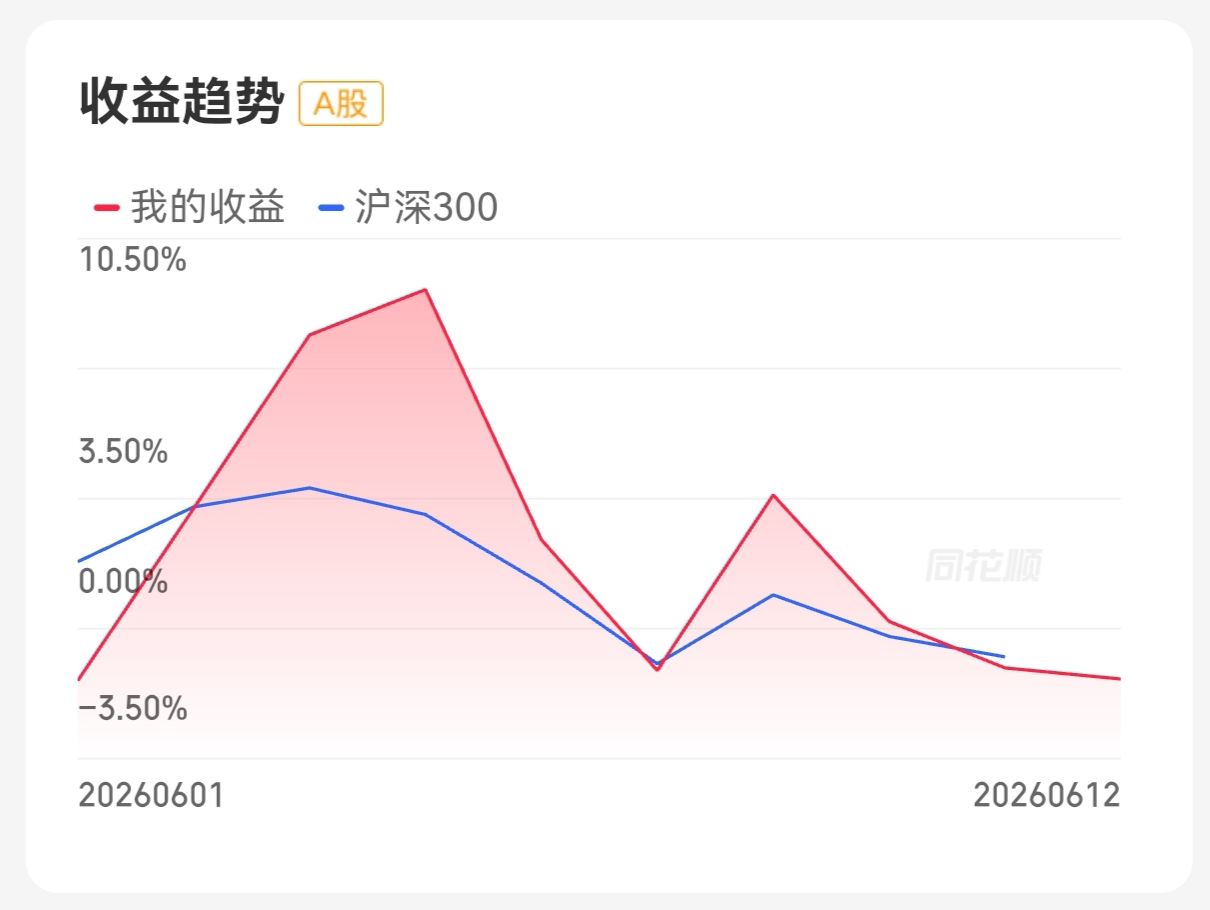
\includegraphics[width=0.85\textwidth]{figures/return_trend.jpg}
    \caption{比赛期间收益趋势图（红线：策略；蓝线：沪深300）}
    \label{fig:return_trend}
\end{figure}

如图\ref{fig:return_trend}所示，收益曲线可以分为四个阶段：(1) \textbf{快速上升期}（6/1--6/4）累计+9.14\%，半导体和光通信板块集体走强，模型选出的高弹性标的贡献显著超额收益；(2) \textbf{集中回撤期}（6/5）单日-6.18\%，同一行业暴露在下跌时同步放大损失；(3) \textbf{震荡修复期}（6/8--6/10），组合在6/9强势反弹但随后回吐，说明持仓仍具有较高Beta；(4) \textbf{除权与收官期}（6/11--6/12），新易盛和天孚通信除权后净值计算更依赖正确的股份调整。整体看，收益曲线不是随机游走，而是清楚反映了“高成长行业集中持仓”的快涨快跌特征。

\subsection{比赛绩效}

\begin{table}[htbp]
    \centering
    \caption{比赛最终绩效}
    \begin{tabular}{lll}
        \toprule
        指标 & 本地计算 & 平台记录 \\
        \midrule
        总收益率 & -1.35\% & $\sim$-1.69\% \\
        最大回撤 & -9.62\% & --- \\
        夏普比率 & 0.25 & --- \\
        超额收益 & -2.75\% & --- \\
        最终仓位 & 99.9\% & --- \\
        \bottomrule
    \end{tabular}
\end{table}

平台显示未实现盈亏约为-\yen16,880.75，加上6/5卖出已实现盈利+\yen3,775.17后，累计总盈亏约为-\yen13,106，与本地计算的-\yen13,197接近。剩余差异主要来自平台手续费、除权因子精度、收盘估值口径和小额现金分红处理。

\subsection{最终持仓分析}

\begin{center}
    \captionof{table}{6月12日收盘持仓（同花顺平台数据）}
    \small
    \begin{tabular}{llrrrrr}
        \toprule
        代码 & 名称 & 成本价 & 收盘价 & 股数 & 盈亏(元) & 涨跌幅 \\
        \midrule
        002384 & 东山精密 & 192.66 & 217.55 & 200 & +4,978 & +12.92\% \\
        300502 & 新易盛 & 487.60 & 506.46 & 280 & +5,280 & +3.87\% \\
        600183 & 生益科技 & 138.03 & 151.28 & 200 & +2,649 & +9.60\% \\
        603986 & 兆易创新 & 470.21 & 481.47 & 200 & +2,253 & +2.40\% \\
        600460 & 士兰微 & 31.53 & 32.15 & 100 & +62 & +1.97\% \\
        300308 & 中际旭创 & 1170.01 & 1149.00 & 300 & -6,304 & -1.80\% \\
        688981 & 中芯国际 & 129.07 & 124.88 & 900 & -3,772 & -3.25\% \\
        002463 & 沪电股份 & 134.84 & 125.20 & 200 & -1,929 & -7.15\% \\
        300476 & 胜宏科技 & 352.00 & 327.21 & 200 & -4,959 & -7.04\% \\
        300274 & 阳光电源 & 174.04 & 148.76 & 200 & -5,055 & -14.52\% \\
        600584 & 长电科技 & 77.13 & 68.92 & 200 & -1,641 & -10.64\% \\
        300394 & 天孚通信 & 311.10 & 280.95 & 280 & -8,443 & -9.69\% \\
        \midrule
        \multicolumn{6}{l}{\textbf{未实现盈亏合计}} & \textbf{-16,881} \\
        \bottomrule
    \end{tabular}
\end{center}

\subsection{比赛深度分析}

\subsubsection{选股有效性：抓住主线但暴露集中}

比赛中最有价值的现象，是模型Top-20高度集中到AI算力和半导体产业链，尤其是新易盛、中际旭创、天孚通信三只光通信/光模块核心标的。这并不是人工指定行业后的结果，而是模型从量价、资金流和估值特征中给出的排序。考虑到这些标的在2024--2026年确实处在AI算力扩张的市场主线中，说明模型至少学到了一类有经济含义的结构性信号。

但是，同一个现象也带来了风险：模型把多个相关股票同时排到前列，组合层面形成了明显的行业集中。行业集中在上行阶段体现为超额收益，6/1--6/4组合累计+9.14\%；在下行阶段则体现为相关性上升后的同步回撤，6/5单日下跌-6.18\%。因此，比赛结果不能简单概括为“选股失败”，更准确的说法是：模型抓住了主线，但没有在策略层对主线拥挤度和行业暴露做约束。

\subsubsection{个股归因：盈利和亏损来自同一逻辑}

最终持仓中，东山精密（+12.92\%）、生益科技（+9.60\%）、新易盛（+3.87\%）和兆易创新（+2.40\%）贡献了主要正收益，它们都与AI硬件、电子制造或半导体景气方向相关。亏损较大的天孚通信（-9.69\%）、胜宏科技（-7.04\%）、长电科技（-10.64\%）同样属于相近链条。也就是说，盈利来源和亏损来源并非两套逻辑，而是同一条高弹性成长主线在不同个股和不同日期上的表现。

这对后续改进很有启发：如果只看单个股票，模型似乎有选对也有选错；但从组合角度看，真正的问题是相关性管理。模型给分越集中，越需要策略层加入行业权重上限、个股权重上限或分数行业中性化，否则Top-N机制会把“相似的高分信号”堆叠成同一个风险因子。

\subsubsection{调仓执行：排序信号与手动交易之间存在偏差}

6/5调仓卖出的9只股票合计实现+\yen3,775盈利，胜率67\%，说明模型并非只会“买入高分股”，在部分持仓退出上也有一定效果。三环集团、澜起科技、华润微等股票在卖出时已经获得正收益，调仓帮助组合锁定了一部分利润。

但实际执行并未严格做到每日小幅换仓，而是在6/5进行了一次较大规模调整。这会带来两个问题：一是调仓行为集中发生在板块波动较大的日期，成交价格更容易受到当日情绪影响；二是策略原本“每日换2只”的低换手设计被改变，组合风险暴露在短时间内发生跳变。后续若进入真实交易，应将预测、下单和持仓同步自动化，至少保证调仓规则与回测规则一致。

\subsubsection{短窗口限制：10天比赛不足以检验长期IC}

本模型的训练标签是T+5收益，策略逻辑也是持有一篮子股票等待排序优势兑现。10个交易日的比赛窗口非常短，且中间只包含两段完整的5日预测周期。短窗口下，收益更容易被一次行业冲击或一次建仓时点主导，统计意义远弱于全年回测。因此，比赛结果只能说明模型在该窗口下的组合暴露和执行效果，不能单独作为模型有效性或无效性的最终证据。

\subsubsection{与基准对比：高弹性主动策略}

根据同花顺收益趋势图（图\ref{fig:return_trend}），策略表现出以下特征：

\begin{table}[htbp]
    \centering
    \caption{策略 vs 沪深300（收益趋势图分析）}
    \begin{tabular}{lcc}
        \toprule
        指标 & 本策略 & 沪深300 \\
        \midrule
        最大涨幅 & $\sim$+10\% & $\sim$+3\% \\
        最终收益 & $\sim$-3\% & $\sim$-1\%至-2\% \\
        波动率 & 高 & 低 \\
        选股超额 & 前期显著 & --- \\
        回撤特征 & 快涨快跌 & 平稳下行 \\
        \bottomrule
    \end{tabular}
\end{table}

策略的收益曲线非常典型地反映了一个\textbf{高弹性主动策略}：上涨时显著跑赢指数，下跌时也明显放大回撤。与沪深300相比，本策略不是低波动增强型策略，而是通过主动选股承担更集中的成长风格风险。比赛最终跑输基准，说明模型输出不能直接等价于可交易组合，必须增加风险预算和组合构建环节。

\noindent\textbf{调仓记录与最终持仓截图}因篇幅较长，请参见附录A和附录B。

% ======================================================================
\section{实验亮点}
% ======================================================================

本实验的主要亮点不在于堆叠复杂模型，而在于把模型目标、特征体系和交易策略尽量对齐。EnsembleAttentionGRU用三个轻量子模型降低预测方差，HybridLoss把数值回归和截面排序同时纳入训练目标，二者共同服务于Top-N选股任务。相比追求更深网络，这种设计更符合金融日频数据低信噪比、小Alpha的特点。

第二个亮点是防泄露和现实约束处理。训练、验证、测试严格按时间划分；标准化参数只由训练集拟合；标签构造与输入窗口严格错位；回测中考虑T+1、涨跌停、手续费、滑点、最小交易单位和除权调整。这些细节不会直接提高模型指标，但决定了结果是否可信。特别是比赛中的除权处理表明，交易分析的质量往往取决于这些看似琐碎的工程环节。

第三个亮点是实验没有停留在回测收益，而是把模拟交易中的失败和偏差纳入分析。验证集+55.02\%说明模型和策略在某些市场环境下有效，比赛-1.35\%则暴露出行业集中、满仓约束和执行偏差。两者结合起来，才能更完整地评估一个量化模型：模型可以提供有效排序，但组合构建和风控才决定收益曲线是否可承受。

% ======================================================================
\section{感悟与思考}
% ======================================================================

\subsection{回测优秀不等于实盘有效——但也不等于模型无效}

2025年验证集+55\%的回测表现，与比赛-1.35\%的实际结果形成了鲜明对比。更合理的理解不是二选一地说“回测是假的”或“比赛只是运气差”，而是承认二者检验的是不同层面：回测包含了模型排序、组合调整和MA60仓位过滤；比赛则在满仓约束下暴露了行业集中和短期波动。

从这次实验看，模型可以作为一个有价值的排序器，但不能单独构成完整交易系统。排序器负责回答“哪些股票相对更值得买”，风控层还必须回答“买多少、是否过于集中、市场状态是否适合买、何时减仓”。缺少后半部分时，即使模型方向大体正确，收益也可能在短时间内被回撤吞噬。

\subsection{数据驱动与风险管理的平衡}

深度学习模型擅长从历史数据中学习模式，但历史模式不等于未来。模型在比赛中自动偏向AI算力链条，说明数据驱动方法可以捕捉市场主线；同时，过度偏向同一主线也说明模型并不会天然理解组合风险。行业集中度约束、单票权重上限、止损线和波动率预警这些“非模型”规则，不是对深度学习的削弱，而是让模型输出可交易化的必要条件。

\subsection{短期比赛的特殊性}

10个交易日的比赛窗口对T+5模型并不充分。即使每个预测信号都具有正期望，10天内也只有很少次数可以重复验证，单次行业冲击足以主导最终收益。因此，比赛结果更适合用于发现执行和风险暴露问题，而不是作为唯一的统计评价。真正评价模型，应结合全年验证IC、测试集衰减和比赛实盘反馈共同判断。

\subsection{主观经验与量化模型的结合}

“易中天”（新易盛、中际旭创、天孚通信）作为AI算力赛道核心标的，模型从数据驱动角度将其推至Top-20前列，说明量价和资金流中确实包含与基本面叙事一致的信息。但主观经验仍有价值：当模型给出一组高度同质的股票时，人可以识别其背后的共同风险因子，并通过行业分散或仓位上限进行修正。理想的流程不是用主观判断替代模型，而是让主观判断约束模型最容易忽略的组合层风险。

\subsection{对量化选股的再认识}

通过本次完整流程，我们对量化选股有了更具体的认识：它的核心不是精确预测某只股票未来价格，而是在截面上持续做出略好于随机的排序。Rank IC为0.05左右看似不高，但只要方向稳定，并通过组合分散和交易规则重复执行，就可能转化为可观收益。与此同时，排序优势并不会自动带来可承受的回撤，策略最终还需要在收益、波动、换手、行业暴露和执行成本之间做工程化权衡。

% ======================================================================
\newpage
\appendix
\section{调仓记录截图}
\label{app:adjustment}

\begin{center}
    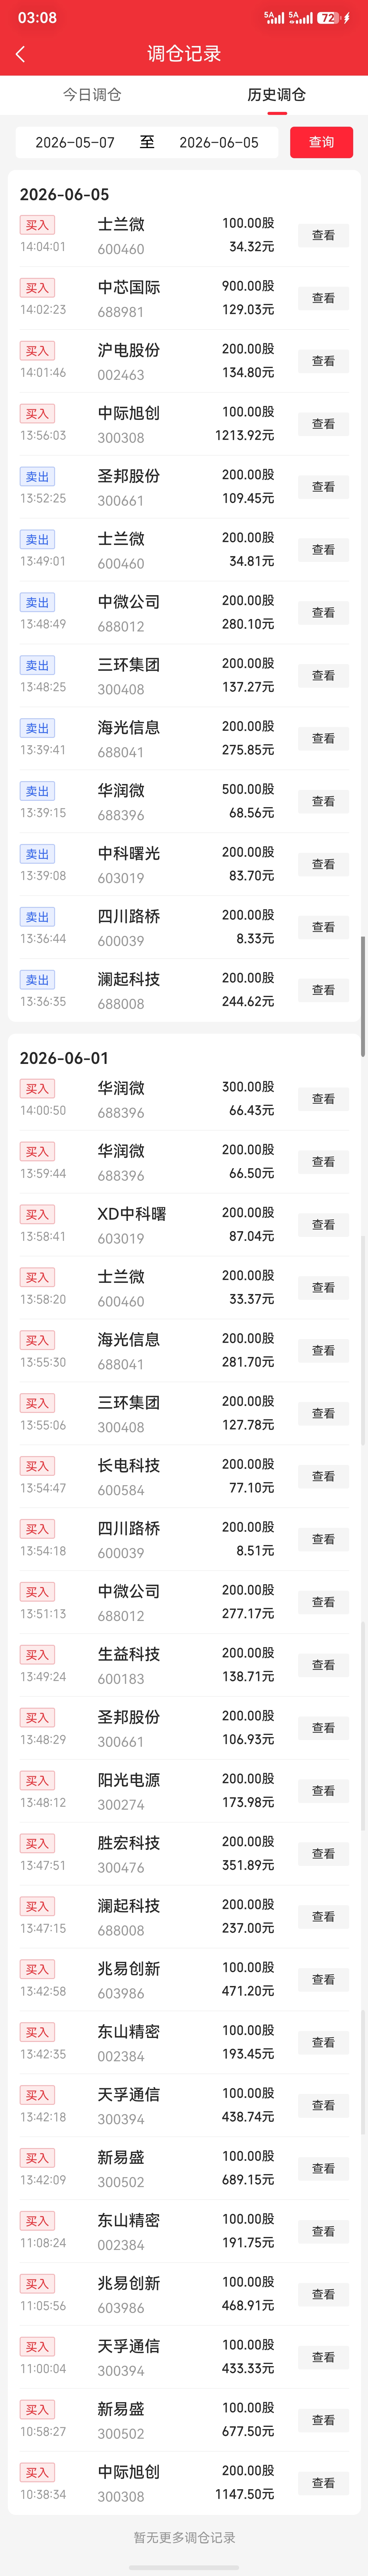
\includegraphics[width=\textwidth,height=0.88\textheight,keepaspectratio]{figures/adjustment_record.jpg}
    \captionof{figure}{同花顺平台完整调仓记录截图}
    \label{fig:adjustment}
\end{center}

\clearpage
\section{持仓记录截图}
\label{app:holding}

\begin{center}
    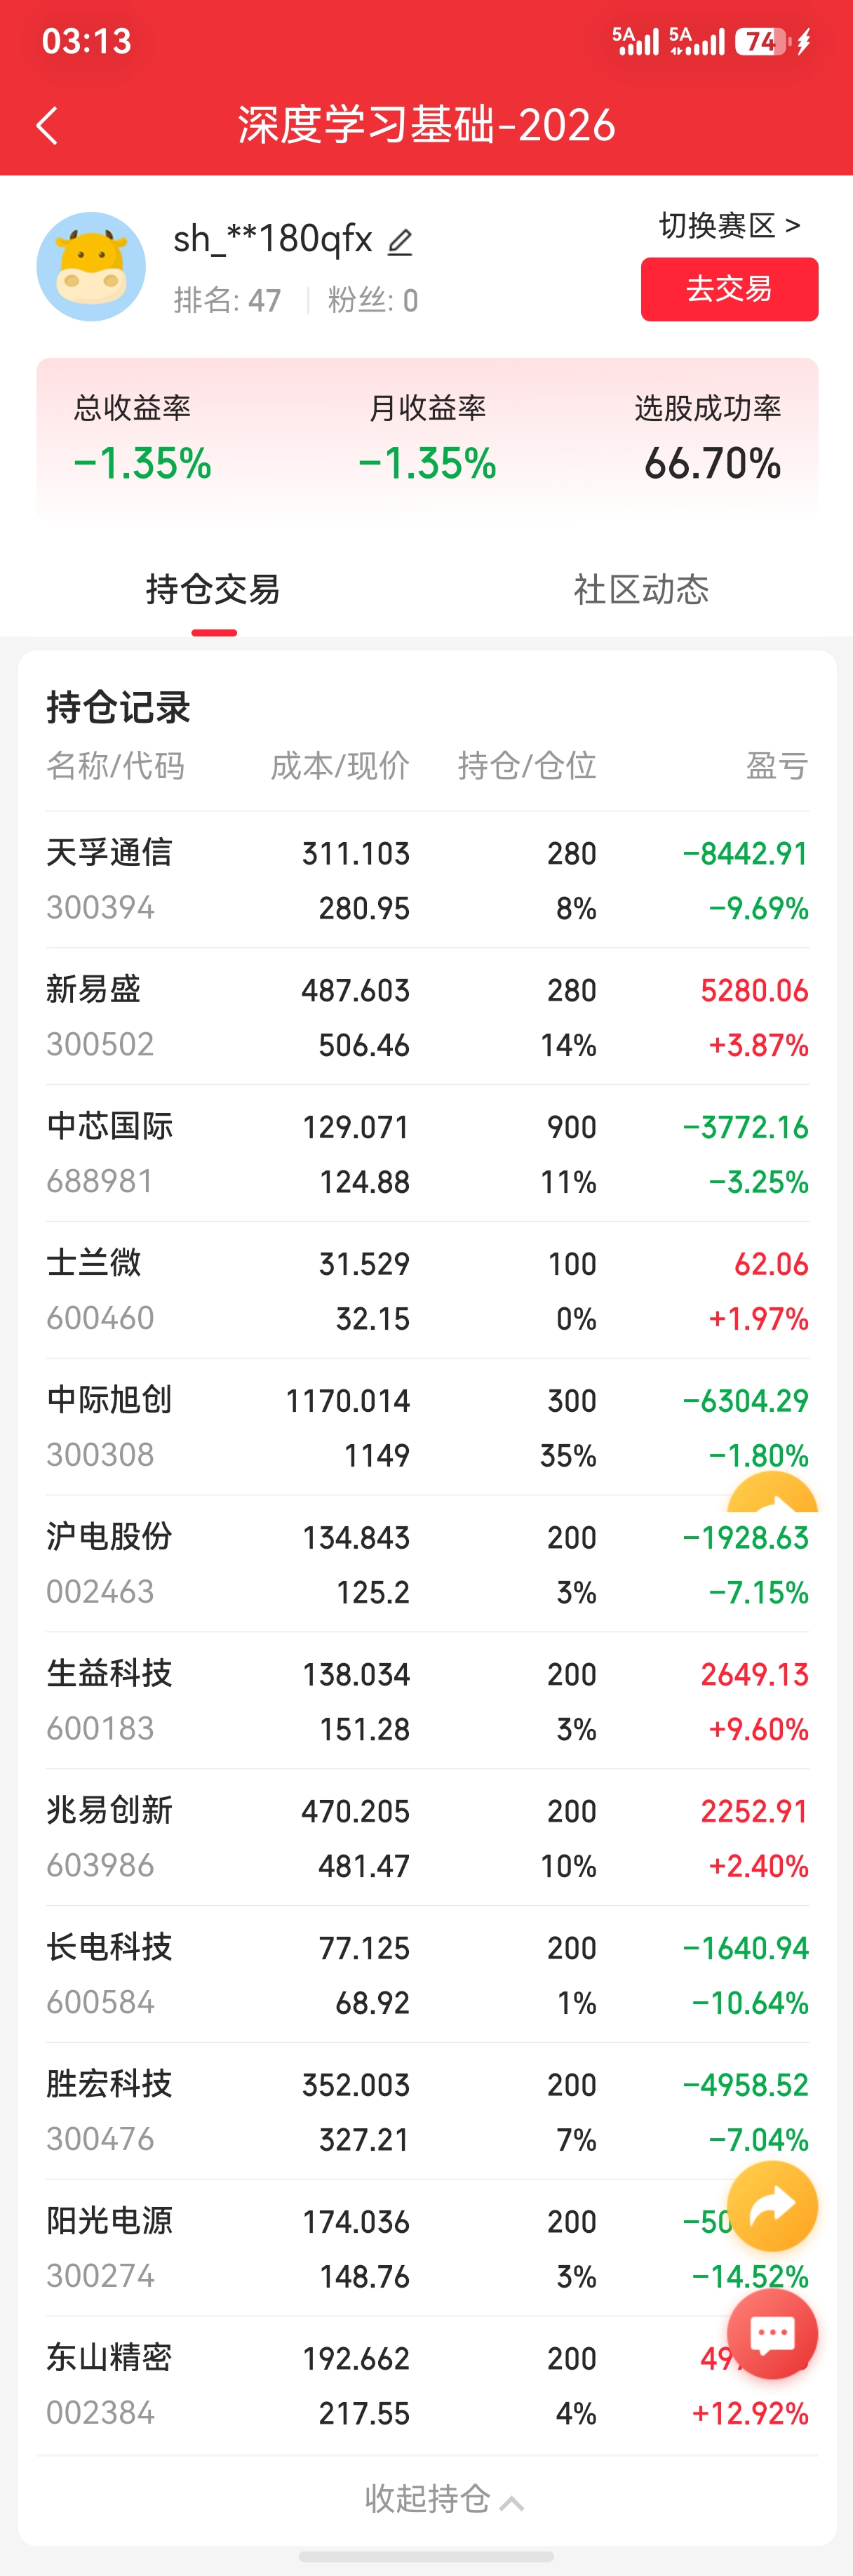
\includegraphics[width=\textwidth,height=0.88\textheight,keepaspectratio]{figures/holding_record.jpg}
    \captionof{figure}{同花顺平台6月12日收盘持仓截图}
    \label{fig:holding}
\end{center}

\clearpage
\section{组员分工}
\label{app:division}

\begin{table}[htbp]
    \centering
    \small
    \begin{tabular}{p{2.2cm}p{3.0cm}p{8.8cm}}
        \toprule
        姓名 & 学号 & 主要分工 \\
        \midrule
        \multirow{3}{*}{王思成} & \multirow{3}{*}{PB23081538} & 数据预处理与特征工程（\texttt{data\_preprocessing.py}） \\
        & & 模型架构设计与实现（\texttt{model.py}, 含 AttentionGRU \& Ensemble） \\
        & & 损失函数设计（HybridLoss）与训练流程（\texttt{train.py}） \\
        \midrule
        \multirow{3}{*}{刘世阳} & \multirow{3}{*}{PB23050876} & 数据集构建与防泄露设计（\texttt{dataset.py}） \\
        & & 回测引擎开发与策略评估（\texttt{backtest.py}） \\
        & & 模拟交易执行、每日预测与比赛调仓 \\
        \midrule
        \multicolumn{2}{l}{\multirow{2}{*}{共同完成}} & 实验报告撰写与结果分析 \\
        \multicolumn{2}{l}{} & 模型迭代优化与超参数调优 \\
        \bottomrule
    \end{tabular}
\end{table}


\end{document}

